%%
%% Automatically generated file from DocOnce source
%% (https://github.com/hplgit/doconce/)
%%

% #define PREAMBLE

% #ifdef PREAMBLE
%-------------------- begin preamble ----------------------

\documentclass[%
oneside,                 % oneside: electronic viewing, twoside: printing
final,                   % draft: marks overfull hboxes, figures with paths
10pt,french]{article}

\listfiles               %  print all files needed to compile this document

\usepackage{relsize,makeidx,color,setspace,amsmath,amsfonts,amssymb}
\usepackage[table]{xcolor}
\usepackage{bm,ltablex,microtype}

\usepackage[pdftex]{graphicx}

% Packages for typesetting blocks of computer code
\usepackage{fancyvrb,framed,moreverb}

% Define colors
\definecolor{orange}{cmyk}{0,0.4,0.8,0.2}
\definecolor{tucorange}{rgb}{1.0,0.64,0}
\definecolor{darkorange}{rgb}{.71,0.21,0.01}
\definecolor{darkgreen}{rgb}{.12,.54,.11}
\definecolor{myteal}{rgb}{.26, .44, .56}
\definecolor{gray}{gray}{0.45}
\definecolor{mediumgray}{gray}{.8}
\definecolor{lightgray}{gray}{.95}
\definecolor{brown}{rgb}{0.54,0.27,0.07}
\definecolor{purple}{rgb}{0.5,0.0,0.5}
\definecolor{darkgray}{gray}{0.25}
\definecolor{darkblue}{rgb}{0,0.08,0.45}
\definecolor{darkblue2}{rgb}{0,0,0.8}
\definecolor{lightred}{rgb}{1.0,0.39,0.28}
\definecolor{lightgreen}{rgb}{0.48,0.99,0.0}
\definecolor{lightblue}{rgb}{0.53,0.81,0.92}
\definecolor{lightblue2}{rgb}{0.3,0.3,1.0}
\definecolor{lightpurple}{rgb}{0.87,0.63,0.87}
\definecolor{lightcyan}{rgb}{0.5,1.0,0.83}

\colorlet{comment_green}{green!50!black}
\colorlet{string_red}{red!60!black}
\colorlet{keyword_pink}{magenta!70!black}
\colorlet{indendifier_green}{green!70!white}

% Backgrounds for code
\definecolor{cbg_gray}{rgb}{.95, .95, .95}
\definecolor{bar_gray}{rgb}{.92, .92, .92}

\definecolor{cbg_yellowgray}{rgb}{.95, .95, .85}
\definecolor{bar_yellowgray}{rgb}{.95, .95, .65}

\colorlet{cbg_yellow2}{yellow!10}
\colorlet{bar_yellow2}{yellow!20}

\definecolor{cbg_yellow1}{rgb}{.98, .98, 0.8}
\definecolor{bar_yellow1}{rgb}{.98, .98, 0.4}

\definecolor{cbg_red1}{rgb}{1, 0.85, 0.85}
\definecolor{bar_red1}{rgb}{1, 0.75, 0.85}

\definecolor{cbg_blue1}{rgb}{0.87843, 0.95686, 1.0}
\definecolor{bar_blue1}{rgb}{0.7,     0.95686, 1}

%\setlength{\fboxsep}{-1.5mm}  % adjust cod_vpad/pro_vpad background box

%% Background for code blocks (parameter is color name)

%% pro/cod_vpad: gives some vertical padding before and after the text
%% (but has more simplistic code than _cod/pro_tight+cod/pro).
%% pro/cod_vpad can be used to enclose Verbatim or lst begin/end for code.
%% pro/cod calls _pro/cod_tight and has very little vertical padding,
%% used to enclose Verbatim and other begin/end for code.
%% (pro/cod is what the ptex2tex program could produce with the
%% Blue/BlueBar definitions in .ptex2tex.cfg.)

\newenvironment{cod_vpad}[1]{
   \def\FrameCommand{\colorbox{#1}}
   \MakeFramed{\FrameRestore}}
   {\endMakeFramed}

\newenvironment{_cod_tight}[1]{
   \def\FrameCommand{\colorbox{#1}}
   \FrameRule0.6pt\MakeFramed {\FrameRestore}\vskip3mm}
   {\vskip0mm\endMakeFramed}

\newenvironment{cod}[1]{
\bgroup\rmfamily
\fboxsep=0mm\relax
\begin{_cod_tight}{#1}
\list{}{\parsep=-2mm\parskip=0mm\topsep=0pt\leftmargin=2mm
\rightmargin=2\leftmargin\leftmargin=4pt\relax}
\item\relax}
{\endlist\end{_cod_tight}\egroup}

%% Background for complete program blocks (parameter 1 is color name
%% for background, parameter 2 is color for left bar)
\newenvironment{pro_vpad}[2]{
   \def\FrameCommand{\color{#2}\vrule width 1mm\normalcolor\colorbox{#1}}
   \MakeFramed{\FrameRestore}}
   {\endMakeFramed}

\newenvironment{_pro_tight}[2]{
   \def\FrameCommand{\color{#2}\vrule width 1mm\normalcolor\colorbox{#1}}
   \FrameRule0.6pt\MakeFramed {\advance\hsize-2mm\FrameRestore}\vskip3mm}
   {\vskip0mm\endMakeFramed}

\newenvironment{pro}[2]{
\bgroup\rmfamily
\fboxsep=0mm\relax
\begin{_pro_tight}{#1}{#2}
\list{}{\parsep=-2mm\parskip=0mm\topsep=0pt\leftmargin=2mm
\rightmargin=2\leftmargin\leftmargin=4pt\relax}
\item\relax}
{\endlist\end{_pro_tight}\egroup}

\usepackage{minted}
\usemintedstyle{default}

\usepackage[T1]{fontenc}
%\usepackage[latin1]{inputenc}
\usepackage{ucs}
\usepackage[utf8x]{inputenc}

% Set palatino as the default font family:
\usepackage[sc]{mathpazo}    % Palatino fonts
\linespread{1.05}            % Palatino needs extra line spread to look nice

\usepackage{lmodern}         % Latin Modern fonts derived from Computer Modern

% Hyperlinks in PDF:
\definecolor{linkcolor}{rgb}{0,0,0.4}
\usepackage{hyperref}
\hypersetup{
    breaklinks=true,
    colorlinks=true,
    linkcolor=linkcolor,
    urlcolor=linkcolor,
    citecolor=black,
    filecolor=black,
    %filecolor=blue,
    pdfmenubar=true,
    pdftoolbar=true,
    bookmarksdepth=3   % Uncomment (and tweak) for PDF bookmarks with more levels than the TOC
    }
%\hyperbaseurl{}   % hyperlinks are relative to this root

\setcounter{tocdepth}{2}  % levels in table of contents

% Tricks for having figures close to where they are defined:
% 1. define less restrictive rules for where to put figures
\setcounter{topnumber}{2}
\setcounter{bottomnumber}{2}
\setcounter{totalnumber}{4}
\renewcommand{\topfraction}{0.95}
\renewcommand{\bottomfraction}{0.95}
\renewcommand{\textfraction}{0}
\renewcommand{\floatpagefraction}{0.75}
% floatpagefraction must always be less than topfraction!
% 2. ensure all figures are flushed before next section
\usepackage[section]{placeins}
% 3. enable begin{figure}[H] (often leads to ugly pagebreaks)
%\usepackage{float}\restylefloat{figure}

% --- fancyhdr package for fancy headers ---
\usepackage{fancyhdr}
\fancyhf{} % sets both header and footer to nothing
\renewcommand{\headrulewidth}{0pt}
\fancyfoot[LE,RO]{\thepage}
% Ensure copyright on titlepage (article style) and chapter pages (book style)
\fancypagestyle{plain}{
  \fancyhf{}
  \fancyfoot[C]{{\footnotesize \copyright\ 2018, Ahmed Ammar. Released under CC Attribution 4.0 license}}
%  \renewcommand{\footrulewidth}{0mm}
  \renewcommand{\headrulewidth}{0mm}
}
% Ensure copyright on titlepages with \thispagestyle{empty}
\fancypagestyle{empty}{
  \fancyhf{}
  \fancyfoot[C]{{\footnotesize \copyright\ 2018, Ahmed Ammar. Released under CC Attribution 4.0 license}}
  \renewcommand{\footrulewidth}{0mm}
  \renewcommand{\headrulewidth}{0mm}
}

\pagestyle{fancy}


% prevent orhpans and widows
\clubpenalty = 10000
\widowpenalty = 10000

% --- end of standard preamble for documents ---


\usepackage[french]{babel}

% insert custom LaTeX commands...

\raggedbottom
\makeindex
\usepackage[totoc]{idxlayout}   % for index in the toc
\usepackage[nottoc]{tocbibind}  % for references/bibliography in the toc

%-------------------- end preamble ----------------------

\begin{document}

% matching end for #ifdef PREAMBLE
% #endif

\newcommand{\exercisesection}[1]{\subsection*{#1}}


% ------------------- main content ----------------------



% ----------------- title -------------------------

\thispagestyle{empty}

\begin{center}
{\LARGE\bf
\begin{spacing}{1.25}
Tuteriel: Apprendre l'Astronomie avec Python
\end{spacing}
}
\end{center}

% ----------------- author(s) -------------------------

\begin{center}
{\bf Ahmed Ammar (\texttt{ahmed.ammar@fst.utm.tn})}
\end{center}

    \begin{center}
% List of all institutions:
\centerline{{\small Faculté des Sciences, Université de Tunis El Manar et Société Astronomique de Tunisie.}}
\end{center}
    
% ----------------- end author(s) -------------------------

% --- begin date ---
\begin{center}
2019
\end{center}
% --- end date ---

\vspace{1cm}


\tableofcontents


\vspace{1cm} % after toc




% !split
\section{Introduction}

% !split
\section{Importation de module et poste d'observateur}
Le module \texttt{PyEphem} est disponible sous le nom \texttt{ephem} qui doit être modifié lors de l’importation en \texttt{ep} pour raccourcir la programmation.
\begin{cod}{cbg_gray}\begin{minted}[fontsize=\fontsize{9pt}{9pt},linenos=false,mathescape,baselinestretch=1.0,fontfamily=tt,xleftmargin=2mm]{python}
from pylab import *
import ephem as ep
obs = ep.Observer()
obs.lon = "18.56406"
obs.lat = "53.09546"
obs.elevation = 133.61
\end{minted}
\end{cod}
\noindent
Les fonctions et structures du module \texttt{ephem } sont appelées dans la fonction \texttt{ep.method()}. Tout d'abord, nous définissons la position de l'observateur (instrument d'observation). Pour ce faire, nous créons la structure appropriée (\texttt{structure = ep.Observer ()}) et remplissons ses champs (\texttt{structure.pole = valeur}).

% !split
\section{Objets et leur localisation}
Tous les objets astronomiques importants tels que le soleil, la lune, les planètes et leur lune peuvent être créés par la structure de \texttt{fonction = ep.nomObjet()}.
\begin{cod}{cbg_gray}\begin{minted}[fontsize=\fontsize{9pt}{9pt},linenos=false,mathescape,baselinestretch=1.0,fontfamily=tt,xleftmargin=2mm]{python}
# Objet
lune = ep.Moon()
\end{minted}
\end{cod}
\noindent
Après avoir créé l'objet, nous pouvons calculer son emplacement actuel en fournissant des informations sur l'observateur, situées dans la structure \texttt{obs} précédemment créée.
\begin{cod}{cbg_gray}\begin{minted}[fontsize=\fontsize{9pt}{9pt},linenos=false,mathescape,baselinestretch=1.0,fontfamily=tt,xleftmargin=2mm]{python}
lune.compute(obs)
\end{minted}
\end{cod}
\noindent
Comme vous pouvez le constater, vous pouvez définir plusieurs observateurs différents et compter les coordonnées de l'objet sélectionné pour différents endroits de la Terre. Cela peut être utile lors de la planification de campagnes d’observation menées par différents observatoires.
% !split
\section{Lecture de coordonnées}

Les coordonnées calculées sont lues à partir des champs de structure d'objet.
\begin{cod}{cbg_gray}\begin{minted}[fontsize=\fontsize{9pt}{9pt},linenos=false,mathescape,baselinestretch=1.0,fontfamily=tt,xleftmargin=2mm]{python}
# coordonnées calculées
print("Position actuelle de la Lune")
print(" ------------------------------ ")
# nous affichons l'ascension droite et la déclinaison
print("RA : ", lune.ra)
print("Dec : ", lune.dec)
# nous affichons l'azimut et l'élévation
print("--------------------------------")
print("Az : ", lune.az)
print ("El : " , lune.alt)
\end{minted}
\end{cod}
\noindent
Les valeurs calculées sont données au format \emph{\textbf{heures: minutes: secondes}} ou \emph{\textbf{degrés: minutes: secondes d'arc}} pour l'heure actuelle UT sur époque 2000.
\begin{cod}{cbg_gray}\begin{minted}[fontsize=\fontsize{9pt}{9pt},linenos=false,mathescape,baselinestretch=1.0,fontfamily=tt,xleftmargin=2mm]{text}
Position actuelle de la Lune
 ------------------------------
RA :  6:18:27.81
Dec :  20:49:04.9
--------------------------------
Az :  197:06:32.3
El :  56:50:39.8
\end{minted}
\end{cod}
\noindent
% !split
\section{Coordonnées en degrés}
Toutes les coordonnées calculées par les procédures du module PyEph sont données en \textbf{radians}. lorsque nous voulons écrire leur valeur, par exemple, les radians sont automatiquement convertis au format approprié (heures, minutes, secondes dans le cas d'une ascension droite ou degrés, minutes, secondes d'arc pour d'autres coordonnées).

Si vous souhaitez utiliser des coordonnées calculées sur un graphique, il est utile de les convertir en degrés à l'aide de la fonction degrés.

\begin{cod}{cbg_gray}\begin{minted}[fontsize=\fontsize{9pt}{9pt},linenos=false,mathescape,baselinestretch=1.0,fontfamily=tt,xleftmargin=2mm]{python}
# coordonnées azimutales en degrés sous forme d'un nombre réel
print(" -------------------------------- ")
print("Az (deg): ", degrees(lune.az))
print("El (deg): ", degrees(lune.alt))
\end{minted}
\end{cod}
\noindent
Azimut et élévation en degrés:
\begin{cod}{cbg_gray}\begin{minted}[fontsize=\fontsize{9pt}{9pt},linenos=false,mathescape,baselinestretch=1.0,fontfamily=tt,xleftmargin=2mm]{text}
--------------------------------
Az (deg):  207.85208210454263
El (deg):  55.334644372169485
\end{minted}
\end{cod}
\noindent

% !split
\section{Villes et à tout moment}
Si nous ne connaissons pas la position exacte de l'observateur et que, simultanément, nous n'avons besoin que des valeurs estimées des coordonnées, par exemple. pour évaluer si un objet donné est visible, nous pouvons utiliser l'une des 122 villes dont les positions ont été enregistrées dans le module \texttt{PyEphem}.
\begin{cod}{cbg_gray}\begin{minted}[fontsize=\fontsize{9pt}{9pt},linenos=false,mathescape,baselinestretch=1.0,fontfamily=tt,xleftmargin=2mm]{python}
# OBSERVATEUR
obs = ep.city("Paris")
print("longitude : ", obs.lon)
print ("latitude : ", obs.lat)
\end{minted}
\end{cod}
\noindent
Nous pouvons attribuer n'importe quelle date et heure à chaque observateur:
\begin{cod}{cbg_gray}\begin{minted}[fontsize=\fontsize{9pt}{9pt},linenos=false,mathescape,baselinestretch=1.0,fontfamily=tt,xleftmargin=2mm]{python}
# PROPRE DATE ET HEURE TU
obs.date = "2019/01/13 10:00:00"
\end{minted}
\end{cod}
\noindent
Il faut seulement se rappeler que les chiffres de la date sont séparés par le signe \texttt{/} et l'heure par deux points.

% !split
\section{Mouvement de la journée solaire - le début du programme}
\begin{cod}{cbg_gray}\begin{minted}[fontsize=\fontsize{9pt}{9pt},linenos=false,mathescape,baselinestretch=1.0,fontfamily=tt,xleftmargin=2mm]{python}
# IMPORTATION
from pylab import *
import ephem as ep
# OBSERVATEUR
obs = ep.city("Warsaw")
# OBJET
soleil = ep.Sun()
# TEMPS
tm = linspace(0 , 24 , 25)
# POLOGNE PAYS POLONAIS
pt = subplot(111 , polar= True )
\end{minted}
\end{cod}
\noindent
% !split
\section{Mouvement du soleil du jour - solstice d'été}
\begin{cod}{cbg_gray}\begin{minted}[fontsize=\fontsize{9pt}{9pt},linenos=false,mathescape,baselinestretch=1.0,fontfamily=tt,xleftmargin=2mm]{python}
# FEUILLE PRINCIPALE
for t in tm :
    # changement de temps
    obs.date = "2014/06/21 %02 d :00:00 "%t
    # on calcule les coordonnées
    sun.compute(obs)
    # coordonnées azimutales - azimut en radians
    az = float(repr(sun.az))
    el = degrees(float(repr(sun.alt)))
    # graphique - on change l'élévation par une distance zénithale
    pt.plot([az], [90 - el], ls =" ", marker= " o ", c =" yellow ", \
    markersize =10)
    # heure locale UTC +2 heures en été
    if el > 0:
        pt.text (az, 90 - el, " %02 d "%(t+2), fontsize =10, \
        ha = 'left' , va = 'center')
\end{minted}
\end{cod}
\noindent
% !split
\section{Mouvement du soleil du jour - solstice d'hiver}
\begin{cod}{cbg_gray}\begin{minted}[fontsize=\fontsize{9pt}{9pt},linenos=false,mathescape,baselinestretch=1.0,fontfamily=tt,xleftmargin=2mm]{python}
    # TRANSFERT HIVERNAL - nous répétons les calculs "en décembre"
    obs.date = "2014/12/22 %02d:00:00" % t
    soleil.compute(obs)
    az = float(repr(soleil.az))
    el = degrees(float(repr(soleil.alt)))
    pt.plot([az], [90 - el], ls ="", marker= "o", c ="blue", \
    markersize =10)
    # heure locale UTC +1 heures en hiver
    if el > 0:
        pt.text (az, 90 - el, "%02d"%(t+1), fontsize =10, \
        ha = 'left' , va = 'center')
#nous limitons la distance zénithale à 90 degrés - horizon
plt.set_rmax(90.0)
# nous plaçons le nord en haut du graphique
plt.set_theta_zero_location("N")
plt.savefig("figs/mvtSoleil.pdf"); plt.savefig ("figs/mvtSoleil.png")
plt.show ()
\end{minted}
\end{cod}
\noindent

% !split
\section{Mouvement du Soleil à la lumière du jour - dessin}


\vspace{6mm}

% inline figure
\centerline{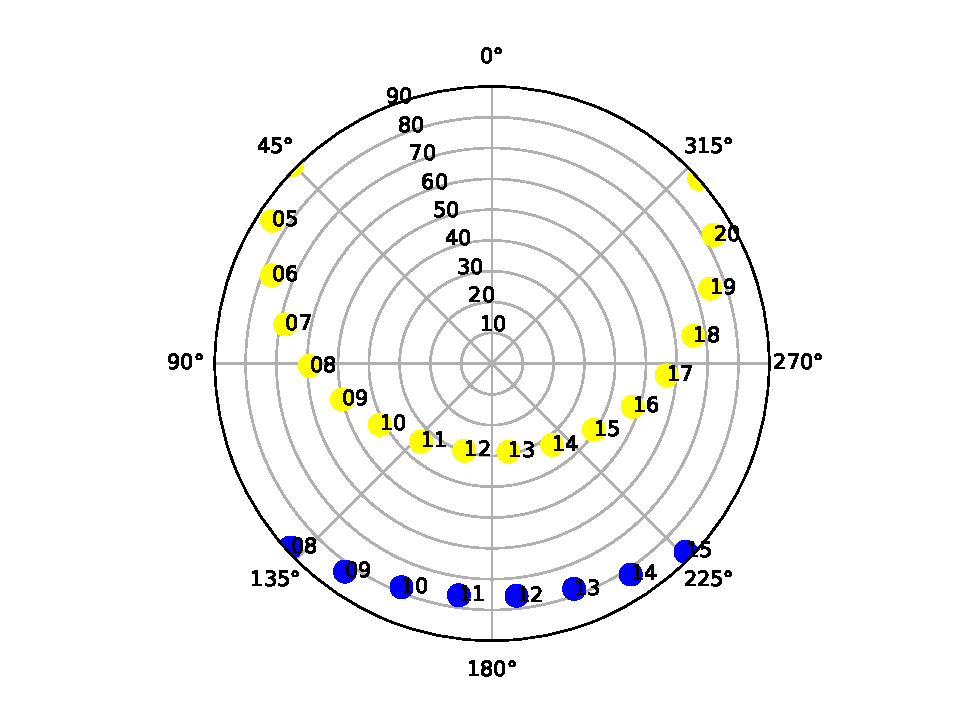
\includegraphics[width=0.9\linewidth]{figs/mvtSoleil.pdf}}

\vspace{6mm}


Le programme vaut également la peine d’ajouter une nouvelle ville, par exemple. \texttt{obs = ep.city("Cairo")}

% ------------------- end of main content ---------------

% #ifdef PREAMBLE
\end{document}
% #endif

